\documentclass{article}
% preamble.tex
\usepackage{amsmath, amsthm, amssymb}
\usepackage{mathtools}
\usepackage{mathabx}
\usepackage{adjustbox}
\usepackage{graphicx}% Required for inserting images
\usepackage{tikz-cd} 
\usepackage{tikz}
\usepackage{comment}
\usetikzlibrary{calc, graphs, positioning, backgrounds, decorations.pathmorphing}
\usepackage{forest}
\usepackage{pgfplots, pgfplotstable}
\usepackage{indentfirst}
\pgfplotsset{compat=1.17}
\usepackage[a4paper,width=150mm,top=25mm,bottom=25mm]{geometry}
\usepackage{fancyhdr}
\pagestyle{fancy}
\usepackage{ifthen}
\usepackage{float}
\usepackage{subcaption}
\usepackage{xkeyval} % Load xkeyval first
\usepackage[colorlinks=true,linkcolor=blue]{hyperref} % Load hyperref with simplified options
\usepackage[dvipsnames]{xcolor}
\usepackage{tcolorbox}
\usepackage{wrapfig}
\usepackage[framemethod=tikz]{mdframed}
\usepackage{atbegshi}% http://ctan.org/pkg/atbegshi


\definecolor{block-gray}{gray}{0.95}
\newtcolorbox{examplesblock}[2][]{%
    grow to right by=-0mm,
    grow to left by=-0mm, 
    opacityback=0,
    frame hidden, boxrule=0pt,
    boxsep=0pt,
    breakable,
    enhanced jigsaw,
    borderline west={2pt}{0pt}{black},
    title={#2\par},
    colbacktitle={black},
    coltitle={black},
    fonttitle={\bfseries},
    attach title to upper={},
    #1,
}

\definecolor{}{gray}{0.95}
\newtcolorbox{codeblock}[2][]{%
    grow to right by=-0mm,
    grow to left by=-0mm, 
    opacityback=0,
    frame hidden, boxrule=0pt,
    boxsep=0pt,
    breakable,
    enhanced jigsaw,
    borderline west={2pt}{0pt}{black},
    title={#2\par},
    colbacktitle={black},
    coltitle={black},
    fonttitle={\large\bfseries},
    attach title to upper={},
}

\titleformat{\chapter}[display]   
{\normalfont\huge\bfseries}{\chaptertitlename\ \thechapter}{20pt}{\Huge}   
\titlespacing*{\chapter}{0pt}{-30pt}{40pt}

\newtheoremstyle{mystyle}%                % Name
  {1pt}%                                     % Space above
  {}%                                     % Space below
  {\normalfont}%                                     % Body font
  {}%                                     % Indent amount
  {\bfseries}%                            % Theorem head font
  {.}%                                    % Punctuation after theorem head
  { }%                                    % Space after theorem head, ' ', or \newline
  {\thmname{#1}\thmnumber{ #2}\thmnote{ (#3)}}%                                     % Theorem head spec (can be left empty, meaning `normal')

  \theoremstyle{mystyle}
\newtheorem*{remark}{Remark}

\NewDocumentCommand{\newframedtheorem}{O{}momo}{%
  \IfNoValueTF{#3}
   {%
    \IfNoValueTF{#5}
     {\newtheorem{#2}{#4}}
     {\newtheorem{#2}{#4}[#5]}%
    }
   {\newfratheorem{#2}[#3]{#4}}
  \tcolorboxenvironment{#2}{#1}%
}
\newmdtheoremenv{theorem}{Theorem}[section]


\newtheorem{corollary}{Corollary}[section]
\newmdtheoremenv{boxcor}{Corollary}[theorem]
\newtheorem{lemma}[theorem]{Lemma}
\newtheorem{prop}[section]{Proposition}
\newtheorem{definition}{Definition}[section] 
%\newtheorem{theorem}{Theorem}[section] 

\newmdtheoremenv{boxdef}{Definition}[section]
\newmdtheoremenv{boxlemma}{Lemma}[section]
\newmdtheoremenv{boxprop}{Proposition}[section]

\newcommand{\here}[2]{\tikz[remember picture]{\node[inner sep=0](#2){#1}}}

\newcommand{\N}{\ensuremath{\mathbb{N}}}
\newcommand{\R}{\ensuremath{\mathbb{R}}}
\newcommand{\Z}{\ensuremath{\mathbb{Z}}}
\newcommand{\Q}{\ensuremath{\mathbb{Q}}}
\newcommand{\C}{\ensuremath{\mathbb{C}}}
\newcommand{\PP}{\ensuremath{\mathbb{P}}}
\newcommand{\F}{\mathcal{F}}

\newcommand{\Real}{\operatorname{Re}}
\newcommand{\Img}{\operatorname{Im}}

\DeclareMathOperator{\spn}{span}
\DeclareMathOperator{\Id}{Id}
\DeclareMathOperator{\essup}{essup}
\DeclareMathOperator{\scrC}{\mathcal{C}}
\DeclareMathOperator{\scrM}{\mathcal{M}}
\DeclareMathOperator{\supp}{supp}
\DeclareMathOperator{\intr}{int}
\DeclareMathOperator{\conv}{conv}
\DeclareMathOperator{\diam}{diam}
\DeclareMathOperator{\ext}{Ext}
\DeclareMathOperator{\dist}{dist}


\newcommand{\inmath}[2]{$#1\in#2$}
\newcommand{\allin}[2]{for all $#1\in#2$}
\newcommand{\isthere}{there exists }

\newcommand{\vectsp}[1]{\mathbf{#1}}
\newcommand{\norm}[1]{\left\lVert#1\right\rVert}
\newcommand{\unitball}[1]{B_{#1}}
\newcommand{\intunitball}[1]{D_{#1}}
\newcommand{\unitsphere}[1]{S_{#1}}

\newcommand{\bigslant}[2]{{\raisebox{.2em}{$#1$}\left/\raisebox{-.2em}{$#2$}\right.}}
\newcommand{\bracket}[2]{\langle #1, #2\rangle}
 % Method of Enrico Gregorio ("egreg")
 % https://tex.stackexchange.com/a/22255/13492:
 \newcommand\restrict[2]{% make the whole thing an ordinary symbol
   \left.\kern-\nulldelimiterspace % automatically resize the bar with \right
   #1% the function
   \littletaller % pretend it's a little taller at normal size
   \right|_{#2}%
   }
 \newcommand{\littletaller}{\mathchoice{\vphantom{\big|}}{}{}{}}

 % Method of Heiko Oberdiek
 % https://tex.stackexchange.com/a/67233/13492
 \makeatletter
 \newcommand*{\scaleddelims}[3]{%
   \ensuremath{%
     \mathpalette{\@scaleddelims{#1}{#2}}{#3}%
   }%
 }   
 \newcommand*{\@scaleddelims}[4]{%
   % #1: left delimiter
   % #2: right delimiter
   % #3: \displaystyle, \textstyle, ...
   % #4: inner formula
   \begingroup
     #3%
     \sbox0{$\m@th#3\vphantom{A}#4$}%
     \setbox2\vbox{\hbox{$\m@th#3#1$}\kern\z@}%
     \setbox4\vbox{\hbox{$\m@th#3#2$}\kern\z@}%
     \setbox6\hbox{$#3\vcenter{}$}%
     \ifx\downharpoonleft#1\relax  
       \let\DelimLeft=L%
     \else\ifx\upharpoonleft#1%
       \let\DelimLeft=L%
     \else\ifx\downharpoonright#1%
       \let\DelimLeft=R%
     \else\ifx\upharpoonright#1%
       \let\DelimLeft=R%
     \fi\fi\fi\fi
     \ifx\downharpoonleft#2\relax
       \let\DelimRight=L%
     \else\ifx\upharpoonleft#2\relax
       \let\DelimRight=L%
     \else\ifx\downharpoonright#2\relax
       \let\DelimRight=R%
     \else\ifx\upharpoonright#2\relax
       \let\DelimRight=R%
     \fi\fi\fi\fi
     \ifx\DelimLeft L%
       \wd2=.6\wd2
     \fi
     \ifx\DelimRight L%
       \wd4=.6\wd4
     \fi
     \ifx\DelimLeft R%
       \sbox2{\kern-.4\wd2\box2}%
     \fi
     \ifx\DelimRight R%
       \sbox4{\kern-.4\wd4\box4}%
     \fi
     \dimen0=\ht0 %
     \advance\dimen0 by -\ht6 %
     \dimen2=\dp0 %
     \advance\dimen2 by \ht6 %
     \ifdim\dimen2>\dimen0 %  
       \dimen0=\dimen2 %
     \else
       \dimen0=\dimen0 %
     \fi
     \dimen2=\ht6 %
     \advance\dimen2 by -\dimen0 %
     \dimen0=2\dimen0 %
     \def\DelimCorr{%  
       \mskip.5\thinmuskip
       \nonscript\mskip.5\thinmuskip
     }%
     \mathopen{%
       \ifx\DelimLeft R\DelimCorr\fi
       \raisebox{\dimen2}{\resizebox{!}{\dimen0}{\box2}}%
       \ifx\DelimLeft L\DelimCorr\fi
     }%
     \begingroup
       #3#4%
     \endgroup
     \mathclose{%
       \ifx\DelimRight R\DelimCorr\fi
       \raisebox{\dimen2}{\resizebox{!}{\dimen0}{\box4}}%
       \ifx\DelimRight L\DelimCorr\fi
     }%
   \endgroup
 }\makeatother
 %

 \newcommand{\restr}[2]{#1\scaleddelims{\kern-0.5\nulldelimiterspace\upharpoonright}{\vphantom{.}}{_{#2}}}
\newcommand{\diff}{\ensuremath{\operatorname{d}\!}}

  % Include the preamble from an external file
\usepackage{algorithm}
\usepackage{algpseudocode}


\difffinecolor{}{gray}{0.95}
\newtcolorbox{codeblock}[2][]{%
    grow to right by=-0mm,
    grow to left by=-0mm, 
    opacityback=0,
    frame hidden, boxrule=0pt,
    boxsep=0pt,
    breakable,
    enhanced jigsaw,
    borderline west={2pt}{0pt}{black},
    title={#2\par},
    colbacktitle={black},
    coltitle={black},
    fonttitle={\large\bfseries},
    attach title to upper={},
}


\AtBeginDocument{\AtBeginShipoutNext{\AtBeginShipoutDiscard}\addtocounter{page}{-1}}
\fancyhead{}
\fancyhead[L]{\text{Imperial UROP 2023}}
\fancyhead[R]{\text{Pantelis Tassopoulos}}

\title{\Huge Imperial College Summer Research \\ 
\huge Under the supervision of Professor Greg Pavliotis}
\author{\Large Pantelis Tassopoulos}
\date{\Large Summer 2023}

\begin{document}


\maketitle
\newpage

\tableofcontents 
\newpage 

\section{Overview}

\subsection{Objectives}

\begin{itemize}
	\item	To examine the existing literature on recent developments in the context of theoretical machine learning that integrate tools from statistical physics and probability theory, i.e., the theory of interacting particle systems.
	\item 	To analyse the approximation quality and trainability of neural networks using algorithms, such as Stochastic Gradient Descent (SGD), informed by such ideas on toy models and examples with real life examples such as the MNIST digit classification dataset.
	\item 	To perform numerical experiments by training neural networks under various circumstances, thereby graining practical insights. 
	\item 	To try and extend results from the literature by attempting to provide theoretical guarantees for accuracy and robustness of machine learning algorithms other than SGD or new insights from numerical simulations. 

\end{itemize}

\subsection{Outcomes}

This Summer Project (UROP) gave me a better insight into cutting-edge research in theoretical machine learning and mathematical optimisation.\\ 

I reviewed the requisite background material in mathematics from reference material, including textbooks and relevant papers. For instance, I read up on topics in probability, namely, martingale inequalities (Doob's and Hoeffman's inequalities in the book of Bremaud entitled 'Probability Theory and Stochastic Processes' \cite{bremaud2020probability}) that Mei et al. in their 2018 paper entitled 'A mean-field view of the landscape of two-layer neural networks' used in proofs of convergence of the SGD dynamics to the evolution of a Partial Differential Equation (PDE) as the hidden layer had an ever-increasing number of nodes, which enabled to perform novel theoretical analyses and provide theoretical guarantees of convergence.\\

I did some additional reading to supplement my understanding of the 2019 papers by Spiliopoulos and Sirgiano entitled 'Mean Field Analysis of Neural Networks: A Law of Large Numbers' and its companion paper \cite{sirignano2019meanfieldanalysisclt}, \cite{sirignano2019meanfieldanalysislln} . I read part of the book entitled 'Markov Processes: Characterisation and Convergence' by Stewart N. Ethier Thomas G. Kurtz \cite{ethier2009markov}, specifically the chapter on weak convergence of probability measures with values on the Skorokhod space $\mathcal{D}_{E[0, \infty)}$, which was necessary for understating the author's arguments on propagation of chaos and analogous convergence arguments. \\

Another crucial component of the project was the emphasis on numerical experiments. They allowed me to demonstrate the validity of theoretical findings and strengthen the case for the arguments presented. Numerical simulations involved training neural networks using existing algorithms from the literature and using insights gained to develop new algorithms. \\

For instance, regarding the above papers by Spiliopoulos, to supplement my understanding and empirically demonstrate claims made in the above paper, I performed numerical simulations by training a family of single-layer neural networks that achieved single-digit classification on the MNIST data set (used for digit classification and is a well-known benchmark for testing models). Upon expanding their hidden layer and training them, I plotted histograms of the distribution parameters which, for sufficiently many hidden nodes, the distribution of node values seemed to stabilise around a fixed bimodal distribution, which is also what the authors reported (while they did not specify the exact nature of the neural network they trained). \\

The project's theme shifted from analysing plain SGD towards understanding the wildly non-convex landscape of the underlying objective/loss function one typically encounters in machine learning applications.\\

In this direction, I demonstrated, among other observations, which can be found on my GitHub page \cite{Tassopoulos_Imperial_Summer_Research_2023} using numerical simulations that Nesterov accelerated gradient descent escaped a 'bad minimum', where SGD got stuck in a loss function that was constructed in \cite{Mei_2018}. \\

This motivated me to generalise further insights gained by examining the dynamics of SGD to momentum-based algorithms, including Nesterov's accelerated Gradient Descent. \\

At that time, I read the 2017 paper by Chaudhari et al. entitled 'Deep Relaxation: partial differential equations for optimising deep neural networks' \cite{Chaudhari2017DeepRP}. They introduced various approaches centred around 'regularising' the loss function. I incorporated both momentum-based methods (including 'restarting' the momentum if the gradient in the change in position was in the direction of the gradient-maximal increase, as was introduced in the 2012 Candes et al. paper entitled 'Adaptive Restart for Accelerated Gradient Schemes' \cite{odonoghue2012adaptiverestartacceleratedgradient}) and regularising the potential (by leveraging the analytical properties of solutions to the Hamilton-Jacobi-Bellman equation) as suggested above to create an algorithm that attempted to escape bad minima.\\

I also revisited the 2023 paper by Andrew Stuart et al. entitled 'Gradient Flows for Sampling: Mean-Field Models, Gaussian, Approximations and Affine Invariance'\cite{chen2023gradientflowssamplingmeanfield} initially suggested by my supervisor to produce another algorithm based on theoretical insights gained from the paper. \\

Furthermore, I read the paper coauthored by my supervisor entitled 'The sharp, the flat and the shallow: Can weakly interacting agents learn to escape bad minima?' \cite{kantas2019sharpflatshallowweakly} I was also led to study the analysis of multiscale algorithms in the literature, e.g. in the Weinan et al. (2005) paper \cite{weinan2005multiscalesde} on the analysis of multiscale methods for SDEs. The authors devised an algorithm that escaped bad minima in a toy example they introduced in the paper. \\

As suggested by my supervisor, I implemented the above algorithms by performing descent on a loss that was a Muller-Brown potential (the canonical example of a potential surface in theoretical chemistry). My instance had a narrow global minimum; SGD would perform poorly and tend to converge to two local minima, of which there were two in a relatively confined domain. For each algorithm mentioned above, I performed random initialisations, ran the algorithms for a fixed number of steps and recorded the final 'losses'. One notable observation is that the implementation of the algorithm in my supervisor’s paper performed noticeably better than the rest, including plain SGD.\\

This research experience presented an excellent opportunity for me to go beyond the scope of material covered in class and explore developments in the literature in a structured and rigorous manner. \\

Please note all the code referenced herein can be found on my personal GitHub page \cite{Tassopoulos_Imperial_Summer_Research_2023} . \\

\newpage
\section{Mean Field Limits of Neural Networks}

\subsection{Background theory}

The process of a neural network 'learning' from data requires solving a complex optimisation problem with millions of variables. This is done by stochastic gradient descent (SGD) algorithms. One can study the case of two-layer networks and derive a compact description of the SGD dynamics in terms of a limiting partial differential equation. This a major insight in \cite{Mei_2018}, where they authors also suggest with their findings that SGD dynamics do not become more complex when the network size increases.\\ 

Now, more formally, one typically encounters, in the context of supervised learning the following: 
\begin{itemize}
	\item Observed data points $ (x_{i},y_{i})_{i\in \N}\subseteq \R^{d}\times \R$, where they are modelled as being independent and indentically distributed (iid).
	\item The $ x\in \R^{d}$ are called \underline{feature vectors} and the $ y\in \R$ the \underline{labels}.
	\item The neural network essentially is a function that depends on some hidden parameters and the feature vector. In the case of a two-layer neural network, the dependence is modelled by: 
		\begin{equation}\label{eq: neural net def}
			\begin{array}{cc}
			\hat{y}:\R^{d}\times \R^{ND}\to \R   \\
			(x;\mathbf{\theta})\mapsto \frac{1}{N}\displaystyle\sum^{N}_{i=1}\sigma_{*}(x;\mathbf{\theta}_{i})     
	     \end{array}
     \end{equation}
		where $ N$ is the number of hidden units (neurons), $ \sigma_{*}:\R^{d}\times\R^{D}\to \R$ an activation function and $\mathbf{\theta} = (\mathbf{\theta})_{i\leq N}$, $\mathbf{\theta}_{i}\in \R^{D}$ are parameters, often $\mathbf{\theta}_{i} = (a_{i}, b_{i}, w_{i})$ for real $ a_{i}, b_{i}, w_{i}$ and $ \sigma_{*}(x;\mathbf{\theta}_{i})=a_{i}=a_{i}\sigma(\bracket{x}{w_{i}}+b_{i})$ for some function $ \sigma:\R\to \R$ (see figure \ref{fig: two layer neural net}).
\end{itemize}


\begin{figure}[H]
    \centering
    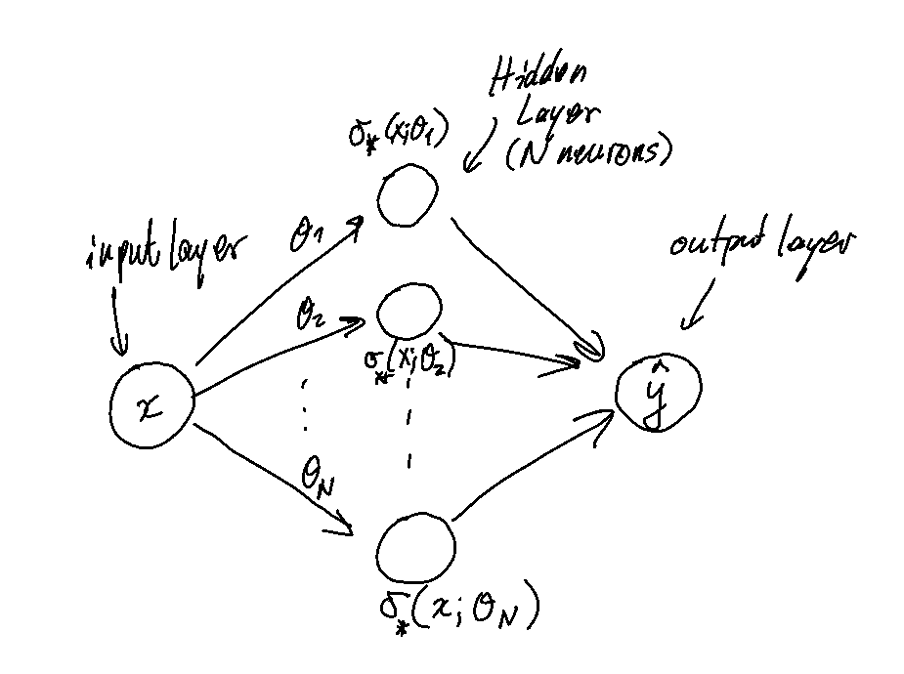
\includegraphics[width=0.6\linewidth]{images/Two-layer-NN.png}
    \caption{ Illustration of a two layer neural network.}
    \label{fig: two layer neural net}
\end{figure}


Naturally, one wants to chose parameters $\mathbf{\theta}$ so as to \underline{minimise} the risk function 
\begin{equation}\label{eq: risk}
	R_{N}(x;\mathbf{\theta}) =\mathbb{E}[\ell(y, \hat{y}(x;\mathbf{\theta}))]
\end{equation}

for a loss function $ \ell:\R\times \R \to \R$, typically and in our case the square loss $ \ell(y-\hat{y})  = (y-\hat{y})^{2}$. This is achieved in practice by stochastic gradient descent summarised below:

\begin{codeblock}{Stochastic Gradient Descent (SGD)}\label{alg: SGD}
\begin{algorithmic}
\State Initialise the parameters $(\mathbf{\theta}_{i})_{i\leq \N} \sim \rho_{0}$, that is according to some initial distribution $ \rho_{0}$.
\While{loss is greater than tolerance}
\State Generate iid sample $ (x, y)\sim \PP$
\For {$1 \leq i \leq N $} 
\State $\mathbf{\theta}_{i}\geqts\mathbf{\theta}_{i}+2s\cdot (y-\hat{y}(x;\mathbf{\theta}))\cdot \nabla_{\mathbf{\theta}_{i}}\sigma_{*}(x;\mathbf{\theta}_i)$ \Comment{square loss is used}
\State Update learning rate $ s$
\EndFor
\EndWhile
\end{algorithmic}

\end{codeblock}

Observe that we have the alternative characterisation of the loss
\begin{equation}\label{eq: loss expanded}
	R_{N}(\mathbf{\theta}) = R_{\#}+ \frac{2}{N}\displaystyle\sum^{N}_{i=1}V(\mathbf{\theta}_{i})+\frac{1}{N^{2}}\displaystyle\sum^{N}_{i,j=1}U(\mathbf{\theta}_{i},\mathbf{\theta}_{j}).
\end{equation} 
where $ V(x; \mathbf{\theta}) = -\mathbb{E}[y\cdot \sigma_(x: \mathbf{\theta})]$, $ U( \mathbf{\theta}_{1}, \mathbf{\theta}_{2}) =\mathbb{E}[\sigma_(x; \mathbf{\theta}_{1})\cdot \sigma_*(x; \mathbf{\theta}_{2})]$ and $ R_{\#}=\mathbb{E}[y^{2}]$ is the risk of the trivial predictor $ \hat{y} = 0$.\\ 

Notice that the collection of weights $  \mathbf{\theta}\in \R^{ND}$ induces a probability measure on $ \R^{ND}$, namely its \textit{empirical measure}:

\begin{equation}\label{eq: empirical measure}
	\hat{\rho}^{(N)} = \frac{1}{N}\displaystyle\sum^{N}_{i=1}\difflta_{ \mathbf{\theta}_{i}} 
\end{equation}

Consider the function on the space of probability measures on $ \R^{D}$, $  \mathcal{P}(\R^{D})$:
\[
\begin{array}{cc}
    R: \mathcal{P}(\R^{D})\to \R \\ 
    \rho \mapsto R_{\#}+ 2 \displaystyle\int V( \mathbf{\theta}) \rho( \diff \mathbf{\theta}) + \displaystyle \int\int U( \mathbf{\theta}_{1}, \mathbf{\theta}_{2}) \rho( \diff \mathbf{\theta}_{1}) \rho( \diff \mathbf{\theta}_{2})   
\end{array}
\]
Observe we can thus express $ R_{N}(\mathbb{\theta}) = R(\hat{\rho}^{(N)})$. Now, performing the SGD algorithm \ref{alg: SGD} for $ k$ steps say (with step size $ s_k = \epsilonilon\cdot \xi(k \epsilonilon)$ for some $ \epsilonilon >0$ and $ \xi: \R_{\geqq 0}\to \R_{\geqq 0}$ sufficiently regular-see \ref{list: reg assumptions}), we obtain the parameters $  (\mathbf{\theta}^{k}_{i\leq N})$ and their respective empirical measures $ \hat{\rho}^{(N)}_k$. In \cite{Mei_2018}, Theorem \ref{thm: mean field nguyen} here, it is shown that for all $ t\geqq 0$, as $ N\to \infty$ and $ \epsilonilon \to 0$ in an appropriate way, the empirical measures $ \hat{\rho}^{(N)}_{t/\epsilonilon}$ converge in the weak sense to some probability measure $ \rho_t$ whose dynamics are governed by the following PDE, which is referred to as \emph{distributional dynamics} (DD) in \cite{Mei_2018}
\begin{equation}
	\begin{array}{ll}
\partial_t \rho_t & =2\xi(t)\, \nabla_{ \mathbf{\theta}}\cdot \Big(\rho_t \nabla_{ \mathbf{\theta}}\Psi( \mathbf{\theta};\rho_t)\Big)\, ,\label{eq:GeneralPDE}\\
\Psi( \mathbf{\theta};\rho) & \equiv V( \mathbf{ \theta})+\int U( \mathbf{\theta}, \mathbf{\theta}')\, \rho(\diff  \mathbf{\theta}') .
\end{array}
\end{equation}

(Note that $\nabla_{ \mathbf{\theta}}\cdot \mathbf{v}( \mathbf{\theta})$ denotes the divergence of the vector field $ \mathbf{v}( \mathbf{\theta})$). This should  be interpreted as an evolution equation in $ \mathcal{P}(\R^D)$.\\

There is rich mathematical literature on the PDE \eqref{eq:GeneralPDE} which was
motivated by the study of interacting particle systems in mathematical physics (see the references in \cite{Mei_2018}). The authors in \cite{Mei_2018} use this to observe that \eqref{eq:GeneralPDE} can be viewed as a gradient flow for the cost function $R(\rho)$ in the space 
$( \mathcal{P}(\R^D),W_2)$, of probability measures on $\R^D$
endowed with the Wasserstein metric.\\

\begin{examplesblock}{Aside:}\label{aside: wasserstein flow}
Regarding Wasserstein flows, I looked through the paper by Y. Chen , et al. \cite{chen2023gradientflowssamplingmeanfield} on Gradient Flows for Sampling and noted down some key insights from their paper(INCLUDE PAPER DETAILS - abstract)
\begin{enumerate}[(a)]
    
	\item 	Given a gradient flow that one has constructed wrt a posterior distribution that one wants to sample from without having an explicit normalization, one can formulate a gradient flow and a system of particles with SDE of the MCKean Vlasov type with FK equation the gradient flow (i.e. the evolution equation of the density). 
	\item 	By making the gradient flow ‘invariant’ under affine reparameterizations (through preconditioning or by suitable choice of metric or energy functional on $\mathcal{P}(\R^d))$, one hope to improve performance of algorithms in the case of highly anisotripic posteriors, if there is an affine transformation that reduces the anisotropic nature of said posterior.
\end{enumerate}
\end{examplesblock}



Recall that Wasserstein distance is defined as
\begin{equation}\label{eq:Wasserstein_dual}
W_2(\rho_1,\rho_2)  = \Big(\inf_{\gamma\in \mathcal{C}(\rho_1,\rho_2)}  \int \| \mathbf{\theta}_1- \mathbf{\theta}_2 \|_2^2 \gamma( \diff  \mathbf{\theta}_1, \diff \mathbf{\theta}_2) \,\Big)^{1/2}. 
\end{equation}

In order to establish that these PDEs indeed describe the limit of the SGD dynamics, we make the following assumptions.
%
\begin{itemize}\label{list: reg assumptions}
%
	\item[{\sf A1.}] $t\mapsto \xi(t)$ is bounded Lipschitz: $\|\xi\|_{\infty}, \|\xi\|_{\text{Lip}}\leq K_1$, with $\int_0^{\infty}\xi(t) \diff  t=\infty$.
%
\item[{\sf A2.}] The activation function $( \mathbf{x}, \mathbf{\theta})\mapsto \sigma_*( \mathbf{x}; \mathbf{ \theta})$ is bounded, with sub-Gaussian gradient: $\|\sigma_*\|_{\infty}\leq  K_2$, $\|\nabla_{ \mathbf{ \theta}}
\sigma_*( \mathbf{X}; \mathbf{\theta})\|_{\psi_2}\leq K_2$. Labels are bounded $|y_k|\leq K_2$.
%
\item[{\sf A3.}] The gradients $\mathbf{\theta}\mapsto \nabla V( \mathbf{\theta})$, $(\mathbf{\theta}_1,\mathbf{\theta}_2)\mapsto \nabla_{\mathbf{\theta}_1}U(\mathbf{\theta}_1,\mathbf{\theta}_2)$  are bounded, Lipschitz continuous 
(namely $\| \nabla_{\mathbf{\theta}}V(\mathbf{\theta}) \|_2$, $\|\nabla_{\mathbf{\theta}_1}U(\mathbf{\theta}_1,\mathbf{\theta}_2)\|_2\leq K_3$, $\|\nabla_{\mathbf{\theta}}V(\mathbf{\theta})-\nabla_{\mathbf{\theta}}V(\mathbf{\theta}')\|_2\leq K_3 \|\mathbf{\theta}-\mathbf{\theta}'\|_2$, $\|\nabla_{\mathbf{\theta}_1}U(\mathbf{\theta}_1,\mathbf{\theta}_2)-\nabla_{\mathbf{\theta}_1}U(\mathbf{\theta}'_1,\mathbf{\theta}_2')\|_2\leq K_3 \|(\mathbf{\theta}_1,\mathbf{\theta}_2)-
(\mathbf{\theta}_1',\mathbf{\theta}_2')\|_2$).
%
\end{itemize}

\begin{theorem}[PM. Nguyen et al. (2018)]\label{thm: mean field nguyen}
Assume that conditions {\sf A1}, {\sf A2}, {\sf A3} hold.
For $\rho_0\in\mathcal{P}(\R^D)$, consider SGD with initialization $(\mathbf{theta}^0_i)_{i\leq N}\sim_{iid}\rho_0$ and step size $s_k = \epsilon \xi(k \epsilon)$. For $t\geq 0$, let $\rho_t$ be the solution of PDE \eqref{eq:GeneralPDE}.
Then, for any fixed $t \geq 0$,  $\hat{\rho}^{(N)}_{\lfloor t / \epsilon \rfloor} \Rightarrow \rho_{t}$ almost surely along any sequence $(N,\epsilon = \epsilon_N)$ such that $N \to \infty$, $\epsilon_N \to 0$, $N/\log (N/\epsilon_N) \to\infty$ and $\epsilon_N \log(N / \epsilon_N)\to 0$.
Further, there exists a constant $C$  (depending uniquely on the parameters $K_i$ of conditions {\sf A1}-{\sf A3}) such that,
for any $f:\R^D\times \R\to\R$, with $\|f\|_{\infty}, \|f\|_{\text{Lip}}\leq 1$, $\epsilon\leq 1$,
%
\begin{align}
%
&\sup_{k \in  [0, T/\epsilon] \cap \N}\Big|\frac{1}{N}\sum_{i=1}^Nf(\mathbf{\theta}^{k}_i)- \int\!
  f(\mathbf{\theta})  \rho_{k\epsilon}(\diff \mathbf{\theta}) \Big| \leq Ce^{CT}\,\text{Err}_{N,D}(z)\, ,\nonumber\\
&\sup_{k \in  [0, T/\epsilon] \cap \N}\big|R_{N}(\mathbf{\theta}^{k})-R(\rho_{k\epsilon})\big| \leq Ce^{CT}\,\text{Err}_{N,D}(z)\, ,
%
\end{align} 
%
with probability $1- e^{-z^2}$ where $\text{Err}_{N,D}(z)$ is given by
\begin{equation}
	\sqrt{1/N\lor \epsilon}\cdot \left[ \sqrt{D + \log N/\epsilon}+z \right]
\end{equation}

\end{theorem}


\begin{theorem}[Doob's martingale inequality]\label{thm: Doob}
	Let $ (\F_{t})_{t\geq 0}$ be a filtration on the probability space $ (\Omega, \F, \PP)$ and $ (M_{t})_{t\geq 0}$ be a continuous martinagle adapted to the filtration $ (\F_{t})_{t\geq 0}$. Let $ p\geq 1$ and $ T>0$. If $\mathbb{E}[|M_{T}|^{p}]<\infty$ and $ \lambda > 0$, then 
	\begin{equation}
		\PP\left(\displaystyle\sup_{t\in [0,T]}|M_{t}|\geq \lambda\right)\leq \frac{\mathbb{E}[|M_{T}|^{p}]}{\lambda^{p}}
	\end{equation}
	
\end{theorem}

\begin{boxlemma}[Hoeffding's Lemma]\label{lemma: Hoeffding}
Let $ (M_{n})_{n\in\N}$ be a martingale adapted to the filtration $ (\F_{n})_{n\in\N}$ such that for some sequence $ c_{1}, c_{2},\cdots$ of real numbers 
\begin{equation}
	\PP(|M_{n}-M_{n-1}|\leq c_{n}) = 1 \quad \text{for all } n\in N.
\end{equation}
Then for all $ x\geq 0$ and all $ n\geq 1$,
\begin{equation}
    \PP(|M_{n}-M_{n-1}|\geq x)\leq 2 \exp \left( -\frac{1}{2}x^{2}\Big/\displaystyle\sum^{n}_{i=1}c_{i}^{2}  \right)
\end{equation}


\end{boxlemma}


\begin{proof}{(Rough Sketch)}
	The conditions {\sf A1} and {\sf A3} guarantee the existence and uniqueness of solutions to the PDE \ref{eq:GeneralPDE}, interpereted in the weak sense. The discrete SGD dynamics $ (\mathbf{\theta}_{i}^{k})_{i\leq N }$ appxorimate the continuous time dynamics. Then the proof becomes technical and the aim is to control error terms incurred when comparing the deviation of the discrete and continuous dynamics in probability. The sub-gaussianity and Lipscitz continuity feature prominently and the tools used to achieve bounds on the the probabilities are mainly Doob's maximal inequality \ref{thm: Doob} and Hoefdding's lemma \ref{lemma: Hoeffding}. 
\end{proof}

The PDE formulation leads to several insights and simplifications. One can exploit symmetries in the data distribution $ \PP$ for instance. If $ \PP$ has rotational symmetry, then one can look for solutions to the PDE problem that share such rotational symmetry, thereby reducing the dimensionality of the problem which facilitates theoretical and numerical analysis. This is manifest in the case of two isotropic Gaussians considered later. Such symmetry cannot be achieved when considering the discrete dynamics since no set of poitns $ \mathbf{\theta}_{1}, \cdots, \mathbf{\theta}_{N}\in \R^{d}$ is invariant under rotations (excluding trivial cases).


\subsection{Centred Isotropic Gaussians}

The authors in \cite{Mei_2018} were interested in numerically testing their PDE framework on the classification problem of Gaussians with the same mean. That is, assume the joint law $ \PP$ of $(\mathbf{x}, y) $ to be:
\begin{equation}
\begin{array}{cc}
& \text{with probability} $ 1/2: y = +1, \mathbf{x}\sim N(0, (1+\Delta)^{2}\cdot\Id_{d})$\\
& \text{with probability} $ 1/2: y = -1, \mathbf{x}\sim N(0, (1-\Delta)^{2}\cdot\Id_{d})$
\end{array}
\end{equation}

For the activation function set $ \sigma( \mathbf{x}; \mathbf{\theta}) = \sigma(\bracket{w}{ \mathbf{x}})$ where $ \sigma$ is a simple piewewise linear activation function.\\

To try and reproduce the findings in \cite{Mei_2018},I implemented the SGD and the asymptotic PDE for the isotropic Gaussian case (SGD for isotropic gaussians with $10^7$ iterations) with $(w_i^0 )_{i\leq\N} \sim_{iid} \rho_0$, where $\rho_0$ is spherically symmetric. More specifically, I ran a monte carlo simulation of the discrete SGD dynamics and recorded the distance of the particles (hidden parameters $ \mathbf{\theta}$) after a set amount of iterations and aggreagated them, producing figure \ref{fig: SGD histogram isotropic Gaussians}. It compares nicely with the last subplot in \ref{fig: Nguyen 2018 isotropic Gaussian simulation}. 

\begin{figure}[H]
\begin{subfigure}{0.5\textwidth}
  \centering
  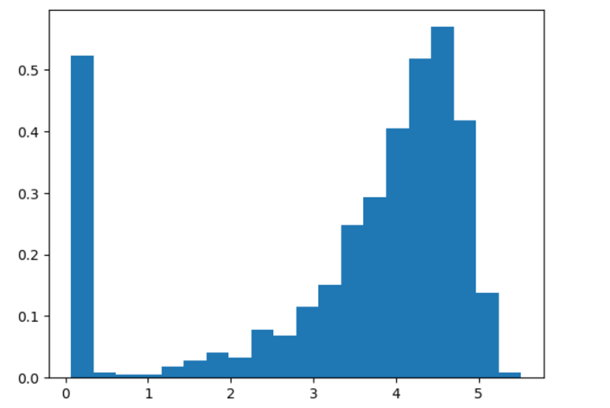
\includegraphics[width=0.8\linewidth]{ images/Nguyen2018-SGD-1.png}
  \caption{fig: SGD histogram for isotropic Gaussians with $ 10^{7}$ iterations.}
  \label{fig: SGD histogram isotropic Gaussians}
\end{subfigure}%
\begin{subfigure}{0.5\textwidth}
  \centering
  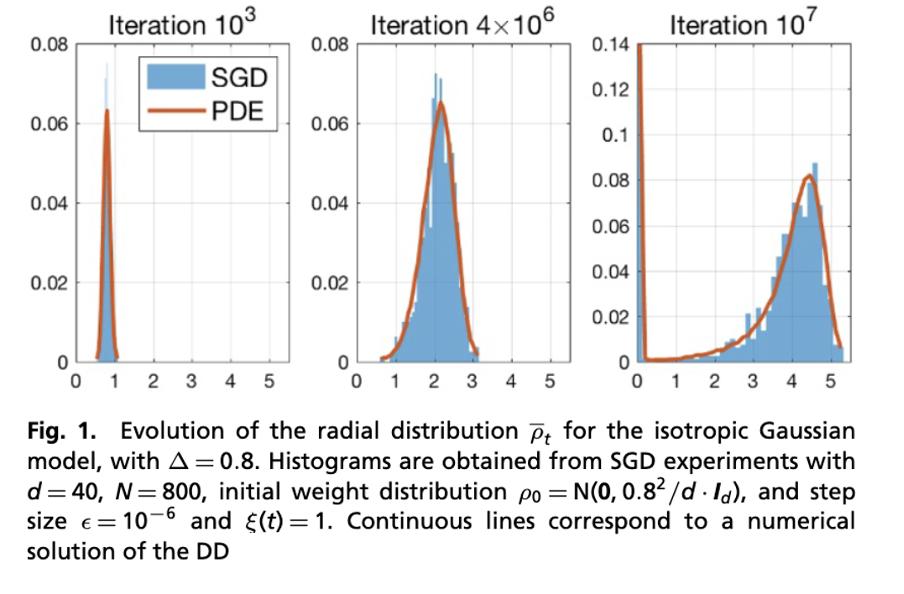
\includegraphics[width=0.8\linewidth]{images/Nguyen2018-paper-numerical-validation-iso-gauss.png}
  \caption{Corresponding simulation in the paper by Nguyen et al.}
  \label{fig: Nguyen 2018 isotropic Gaussian simulation}
\end{subfigure}
\caption{Isotropic Gaussian SGD simulation.}
\label{fig:  isotropic gaussians SGD}
\end{figure}

•	‘I think it would be useful to focus on the numerical experiments, particularly the study of the mean field limit. Mei, Montanari and Nguyen (PNAS, 115(33) 2018)’
•	 ‘Can you please also have a look at the Vanden Eijnden et al paper, in particular the example with radially symmetric functions? What I would like us to study is the possible non-uniqueness of stationary states for the mean field PDE that is derived in the paper by Mei et al.’
•	Managed to implement the PDE in python after optimizing the code (vectorizing, parallelizing) and obtained the following for the distributional dynamics (corresponding to $10^7$ SGD iterations):
•	(DD plot isotropic gaussians)

\begin{figure}[H]
    \centering
    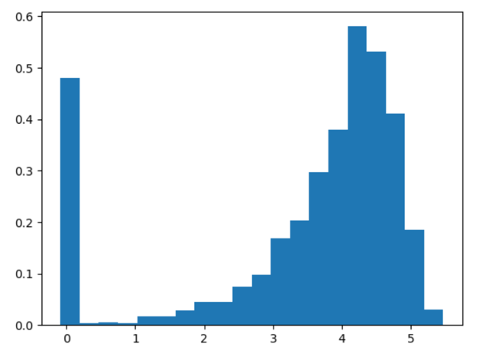
\includegraphics[width=0.6\textwidth]{images/Nguyen2018-SGD-2.png}
    \caption{ caption}
    \label{fig: label of figure}
\end{figure}

	I examined numerically the case of failure of sgd given two initializations motivated by the theory developed in the 2018 paper of Mei et al.
o	Observed slight difference in simulated risk for initialization with kappa = 0.4
 
    \begin{figure}[H]
\begin{subfigure}{0.5\textwidth}
  \centering
  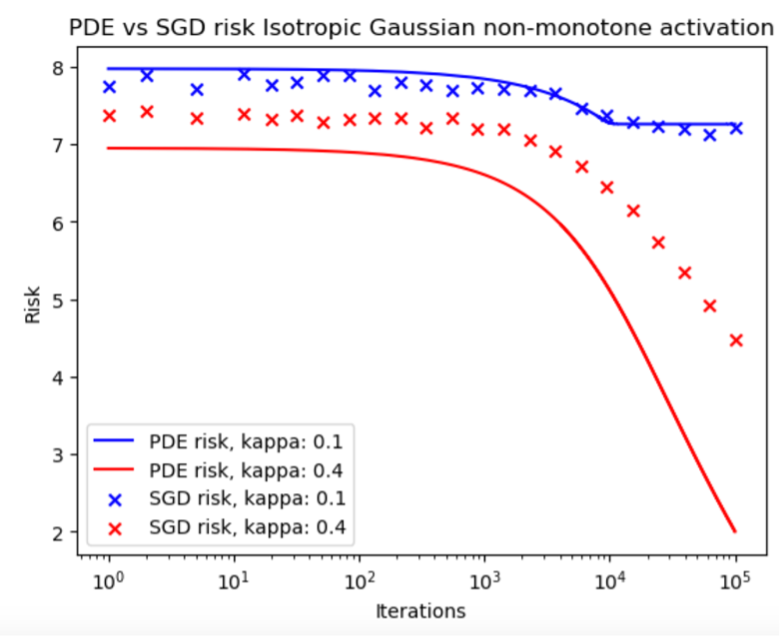
\includegraphics[width=0.8\linewidth]{images/NGuyen2018-pde-sgd-risk-iso-gauss-non-mon.png}
  \caption{ caption}
  \label{fig: description}
\end{subfigure}%
\begin{subfigure}{0.5\textwidth}
  \centering
  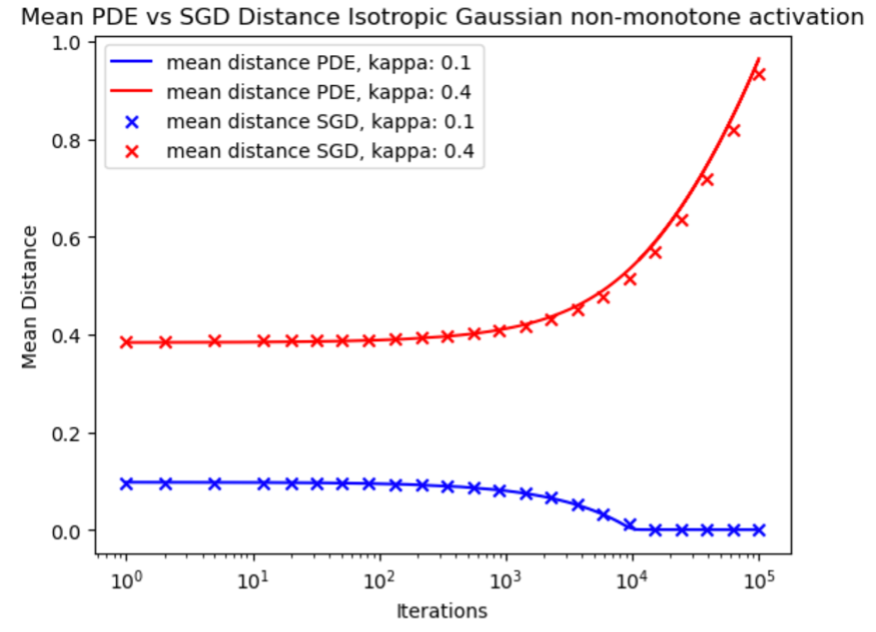
\includegraphics[width=0.8\linewidth]{images/NGuyen2018-pde-sgd-iso-gauss-non-mon.png}
  \caption{ caption}
  \label{fig:  description}
\end{subfigure}
\caption{ caption}
\label{fig:  label}
\end{figure}

•	Implemented code for sgd and pde simulations of risk for the non-isotropic Gaussian case of failure of sgd given two initializations motivated by the theory developed in the 2018 paper of Mei et al.
o	PDE simulations reproduce the numerical findings in the paper, but sgd runs fail to match the pde profiles exactly:
     \begin{figure}[H]
 \begin{subfigure}{0.5\textwidth}
   \centering
   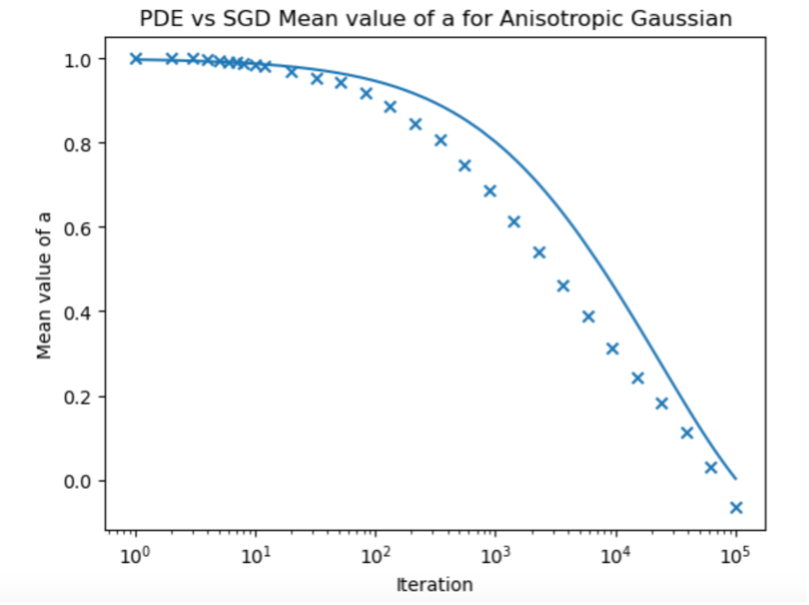
\includegraphics[width=0.8\linewidth]{images/NGuyen2018-pde-sgd-gauss-anisotropic.png}
   \caption{ caption}
   \label{fig: description}
 \end{subfigure}%
 \begin{subfigure}{0.5\textwidth}
   \centering
   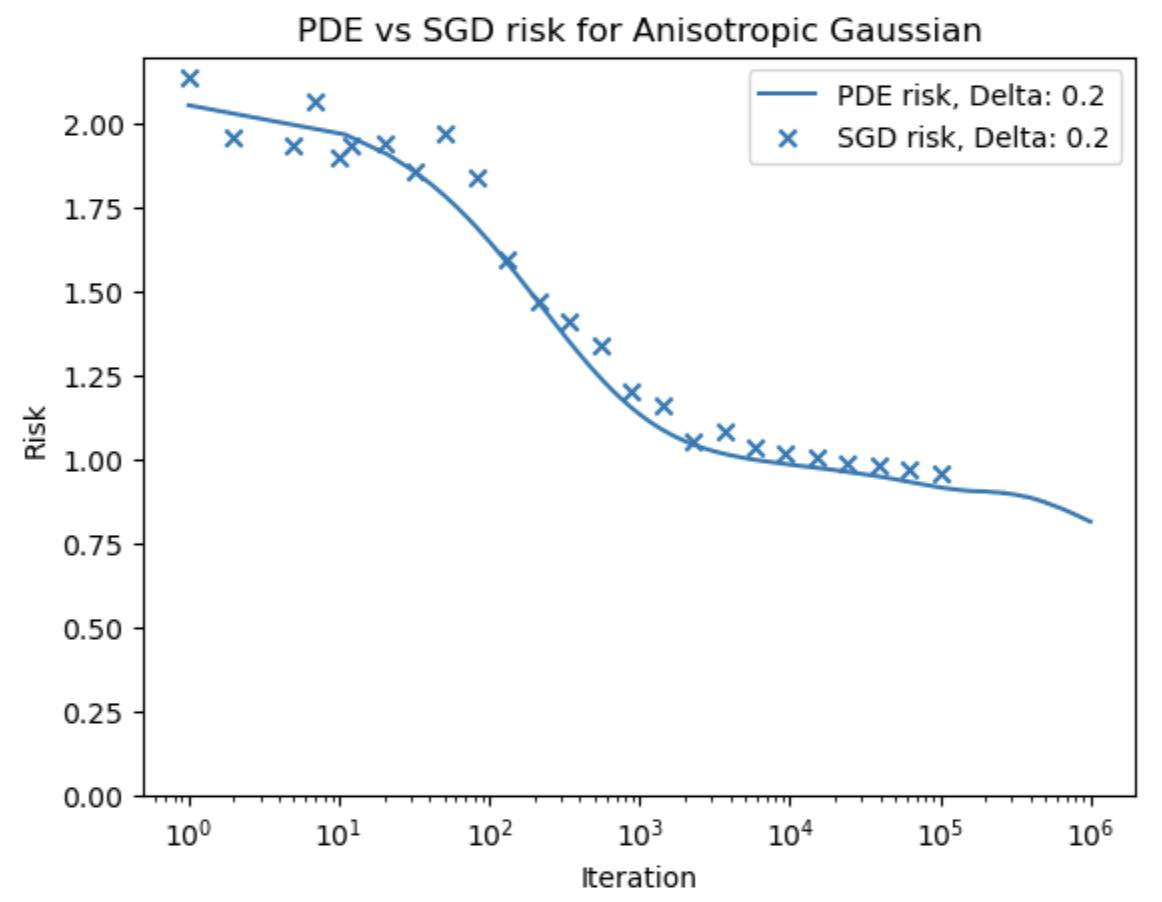
\includegraphics[width=0.8\linewidth]{images/NGuyen2018-pde-sgd-risk-gauss-anisotropic.png}
   \caption{ caption}
   \label{fig:  description}
 \end{subfigure}
 \caption{ caption}
 \label{fig:  label}
 \end{figure} 

 
•	Studied the proofs for the propagation of chaos and the mean-field limit of the distribution of neural network weights in the 2019 paper of Spiliopoulos and Sirgiano  entitled ‘Mean Field Analysis of Neural Networks: A Law of Large Numbers’ and its companion paper \cite{sirignano2019meanfieldanalysislln}, \cite{sirignano2019meanfieldanalysisclt}.
•	Also did some background reading to supplement my understanding of the above papers of a book entitled ‘Markov Processes: Characterization and Convergence’ by Stewart N. Ethier, Thomas G. Kurtz, specifically the chapter on weak convergence of probability measures with values on the Skorokhod space $D_E[0,infinity)$.

I read the companion paper of Spiliopoulos (2019) where the authors proved a CLT for a one-layer neural net. My question is whether the convergence of the empirical measure, up to scaling, is proved in the dual of some Sobolev space. I imagine this is a rather weak form of convergence.
•	Furthermore, regarding the paper of Spiliopoulos (2019) on the LLN for the one-layer neural net, I implemented a single-digit classifier with the architecture satisfying the assumptions made in the paper and was able to reproduce the distribution of parameters in the paper.

\begin{figure}[H]
    \centering
    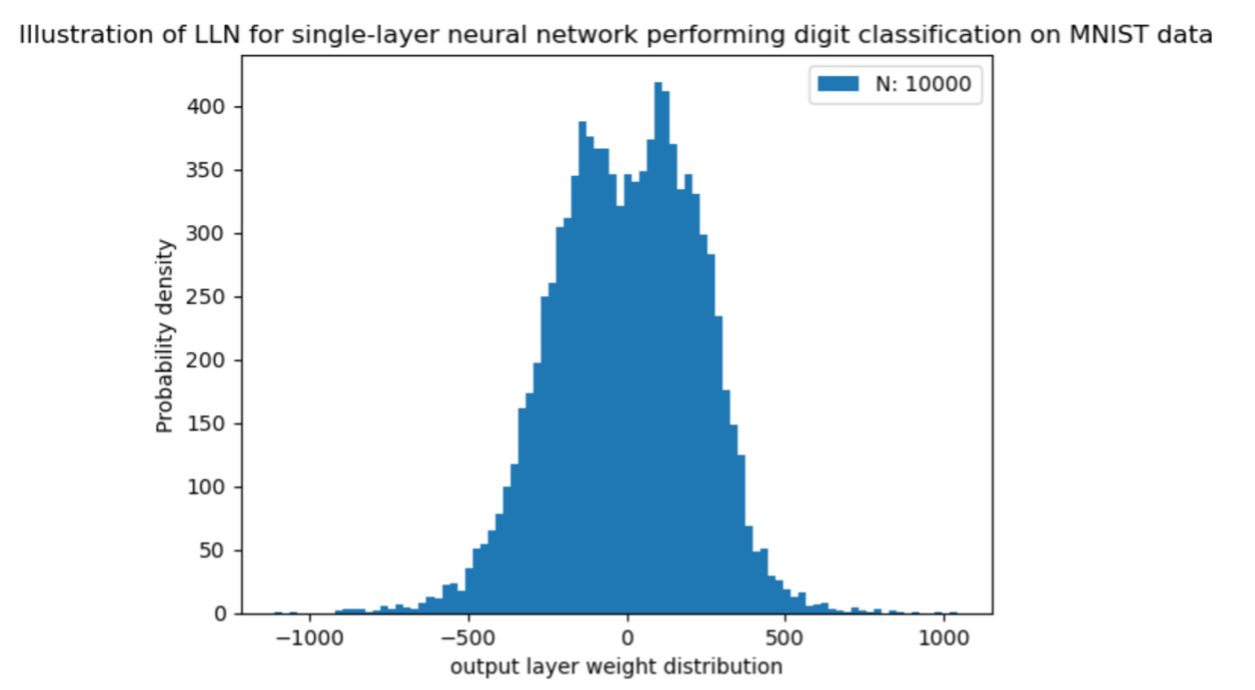
\includegraphics[width=0.8\textwidth]{images/Spiliopoulos2019-LLN-singleNN-mnist.png}
    \caption{ caption}
    \label{fig: label of figure}
\end{figure}

•	Does the empirical measure of the particles converging to a deterministic measure automatically yield the propagation of chaos? It seems these terms are used interchangeably, though the latter is not really elaborated upon.  


\section{Non-convex landscape}

\subsection{Approaches}
\subsubsection{Potential regularisation}
	I have read your paper on shallow minima: ‘The sharp, the flat and the shallow: Can weakly interacting agents learn to escape bad minima?’
o	I also looked at the algorithms and their justifications in the Weinan et al. (2005) paper on the analysis of multi-scale methods for SDEs
o	It seems to me the algorithm introduced in the paper corresponds to a discretization of the dynamics of gradient descent against a potential with an l-2 penalty and a regularized version of the original potential $\Phi$, using the method introduced by Chaudhari et al. (2018).


\subsection{Applications}

\subsubsection{Muller Brown Potential}

•	Muller-Brown potential analysis:
o	- Most algorithms on the MB potential get stuck equally on two local minima, i.e. the global one (which is narrow) and the one with the next smallest local minimum
o	- Convolving with a solution to the heat equation does not improve performance as the narrow steep global minimum (as seen from the plot) is smeared out first thus giving no hope of real convergence, unless the algorithms is lucky with the initialisation
o	- The Hom-MF-SGLD works surprisingly well against all others since it performs a gradient flow of a regularised potential, where regularisation is done at the level of the gibbs measure
o	- Idea, sample points (to initialise GD) more judiciously, i.e. with gibbs measure (inspired by Andrew Stuart's paper ) by performing a gradient flow and use that 'educated guess as the initialisation of a gd algorithm. (e.g. Wasserstein gradient flow, i.e. sgd on log of Gibbs measure of potential, or affine invariant Wasserstein)
o	- This idea seems to perform better that all algorithms except the MF-Hom-SGLD algorithm
o	- Regularising using the HJB equation (essentially performed in the MF-Hom SGLD algorithm) is better suited to minima that are narrower compared to regularisation with the heat equation that destroys such peaks first (due to large curvature)
o	- Tried regularising wrt soln of HJB equation directly and apply nesterov's accelerated gd algorithm with gradient restarting


\begin{figure}\centering
\subfloat[legend]{\label{a}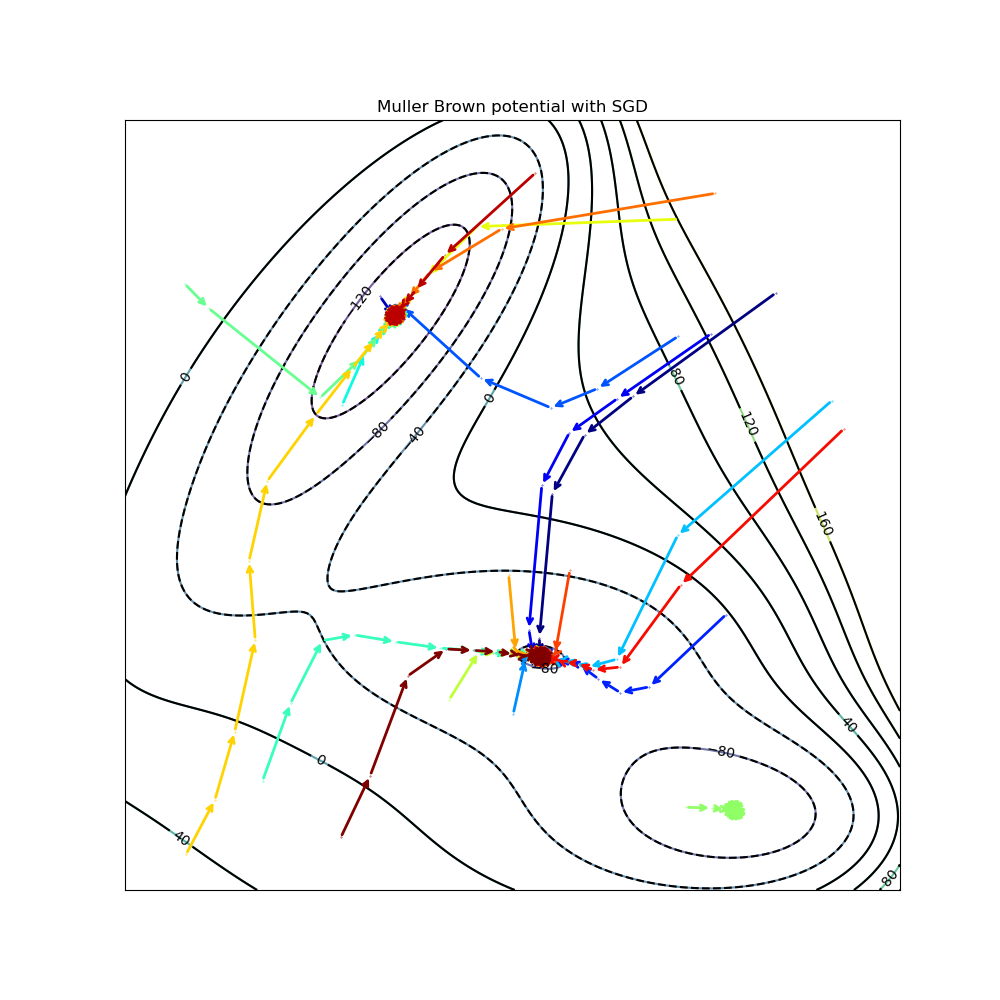
\includegraphics[width=.45\linewidth]{images/MullerBrown-SGD.png}}\hfill
\subfloat[legend]{\label{b}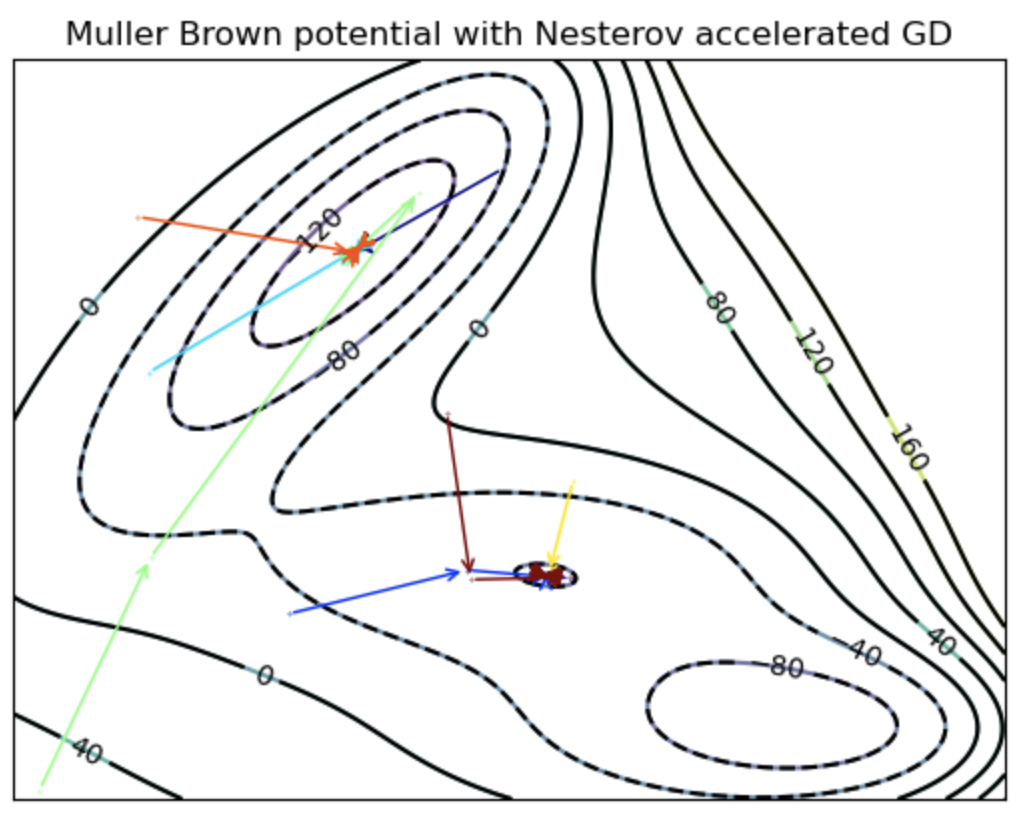
\includegraphics[width=.45\linewidth]{images/MullerB-NesterovSGD.png}}\par 
\subfloat[legend]{\label{c}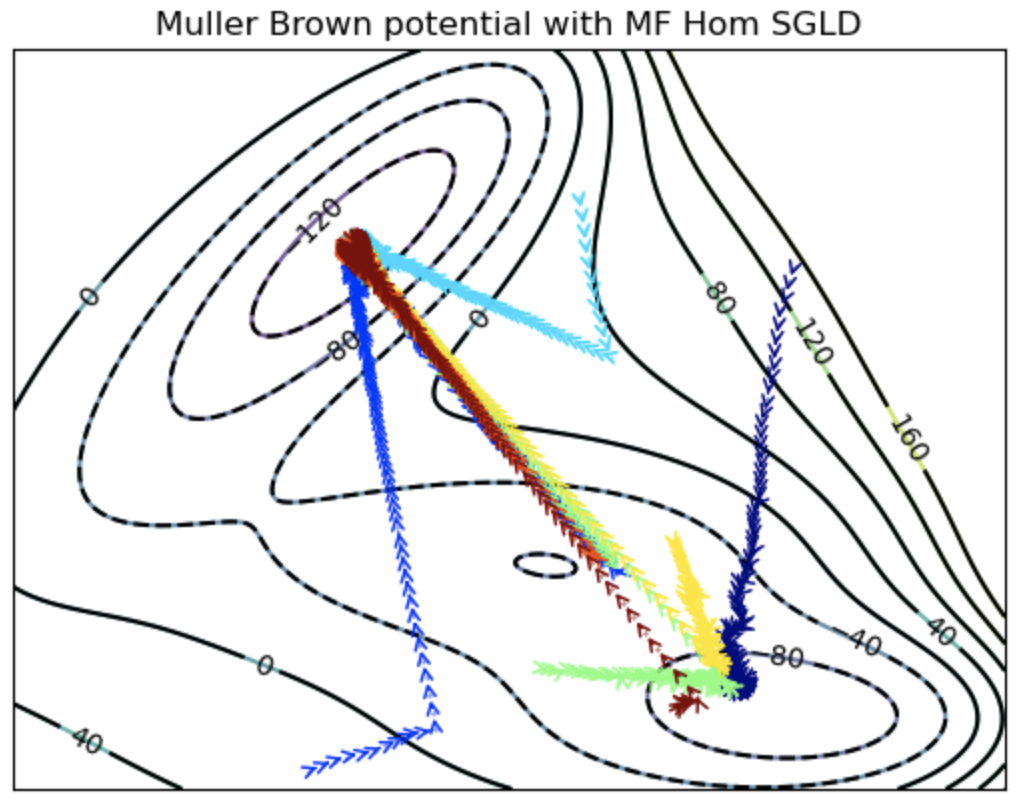
\includegraphics[width=.45\linewidth]{images/MullerBrown-HomSGLD.png}}
\caption{my fig}
\label{fig}
\end{figure}


    \begin{figure}[H]
\begin{subfigure}{0.5\textwidth}
  \centering
  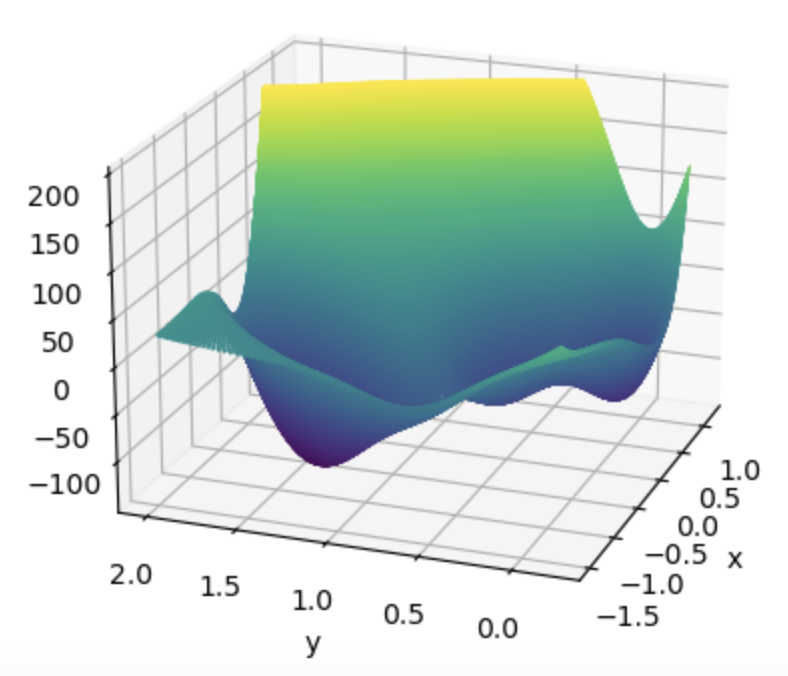
\includegraphics[width=0.8\linewidth]{images/MullerB-potential-plot-3d.png}
  \caption{ caption}
  \label{fig: description}
\end{subfigure}%
\begin{subfigure}{0.5\textwidth}
  \centering
  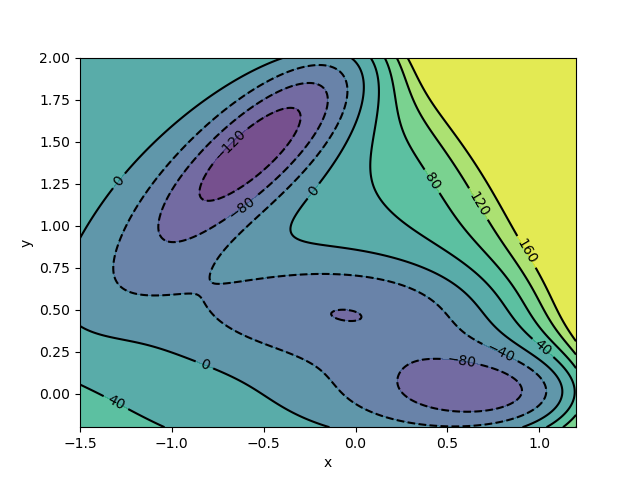
\includegraphics[width=0.8\linewidth]{images/MullerB-contour-with-grad-field.png}
  \caption{ caption}
  \label{fig:  description}
\end{subfigure}
\caption{ caption}
\label{fig:  label}
\end{figure}

\begin{codeblock}{Nesterov SGD on Muller Brown Potential}
\begin{lstlisting}[language=Python]
import numpy as np
#Nesterov Potential 
n = 256
x = np.linspace(-1.5, 1.2, n)
y = np.linspace(-0.2, 2, n)
X, Y = np.meshgrid(x, y)

intervals = np.arange(1, 1e5, 20)

ntraj = 1000
# Initialize holder for trajectories
colors = plt.cm.jet(np.linspace(0,1,np.minimum(ntraj, 7)))
minima_nesterov = []
for j in tqdm(range(ntraj)):
    points_x, points_y = train_nesterov(intervals,
    learning_rate = 1e-4, a = 1, tolerance = 1e-5)
    minima_nesterov.append(MB_potential(points_x[-1],points_y[-1]))
    if j <=6: 
        plt.scatter(points_x, points_y, color = colors[j], s = 0.1)
        for i in range(len(points_x)-1):
            plt.annotate('', xy =[points_x[i+1],
	    points_y[i+1]], xytext= [points_x[i], points_y[i]],
                         arrowprops={'arrowstyle': '->', 'color': colors[j],  'lw': 1},
                         va='center', ha='center')

plt.contour(X, Y, vMB_potential(X, Y).clip(max=200), 8,
alpha=.75, cmap='viridis')
C = plt.contour(X, Y, vMB_potential(X,Y).clip(max=200), 8)
plt.title('Muller Brown potential with Nesterov accelerated GD')
plt.clabel(C, inline=1, fontsize=10)
plt.xticks([])
plt.yticks([])
#plt.legend()    
\end{lstlisting}
    
\end{codeblock}



\subsubsection{$ 3-$d spin model analysis}

•	Implemented gaussian kernel-approximation using SGD to 3-spin model, vanilla version and implemented an algorithm where no new sampling was necessary due to the network parameters and inputs having the same constraint.
•	Read the van Eijnden paper and studied the proofs of asymptotic convergence to a gradient flow in the mean field limit and how this is preferable due to the convexification of the loss (as a functional of measures).
•	Was not able to implement the gradient flow numerically suggested in equation (140) of the van Eijnden 2018 paper. 

\begin{figure}[H]
\begin{subfigure}{0.5\textwidth}
  \centering
  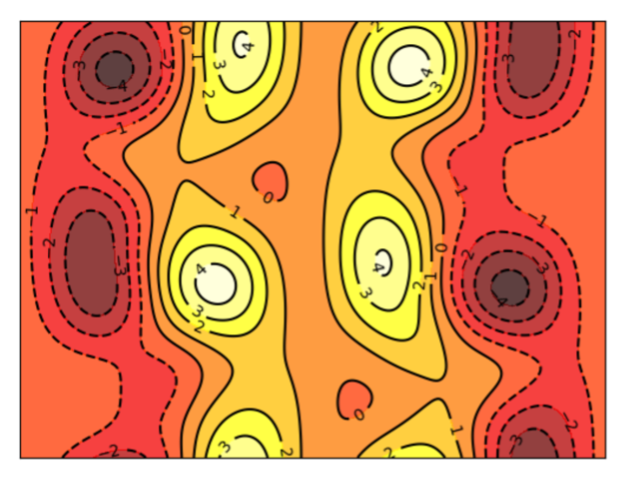
\includegraphics[width=0.8\linewidth]{images/Eijnden2018-heatmap-3dspin.png}
  \caption{ caption}
  \label{fig: description}
\end{subfigure}%
\begin{subfigure}{0.5\textwidth}
  \centering
  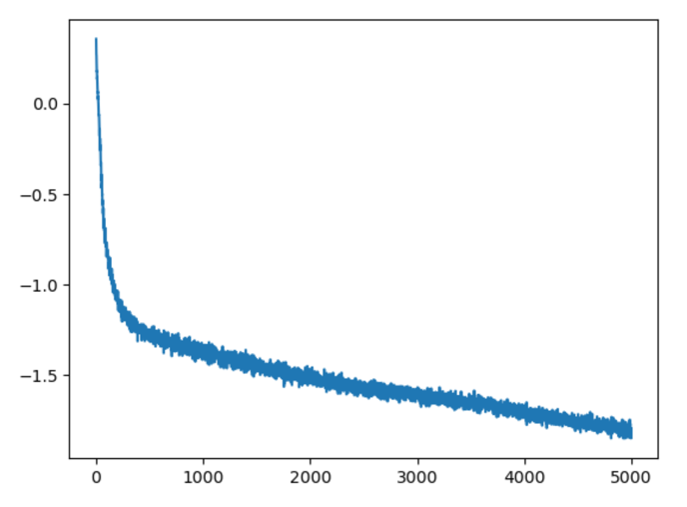
\includegraphics[width=0.8\linewidth]{images/Eijnden2018-loss.png}
  \caption{ caption}
  \label{fig:  description}
\end{subfigure}
\caption{ caption}
\label{fig:  label}
\end{figure}


\subsection{Week 8-10}

I have implemented second-order methods, namely, Nesterov accelerated gradient descent and ‘Discretized mean field SGLD with homogenization’ as conceived in your paper entitled ‘The sharp, the flat and the shallow: Can weakly interacting agents learn to escape bad minima?’. I also came across a paper entitled ‘ACCELERATING SGD WITH MOMENTUM FOR OVER-PARAMETERIZED LEARNING’ by Liu and Belkin, where the authors claim that Nesterov SGD with any parameter selection does not in general provide acceleration over ordinary SGD’. There the authors come up with a modified algorithm which they call ‘Momentum-added stochastic solver (MaSS)’. I have made the following observations:
 
•	For the Isotropic Gaussian learning problem in the 2018 paper by Mei et al.
o	Nesterov-accelerated GD beats plain SGD, as expected
 
 
•	Anisotropic Gaussian learning problem in the 2018 paper by Mei et al.
o	Here Nesterov accelerated SGD performs the best, outperforming plain SGD, and while in the beginning, the MF-HomSGLD matches the performance of plain SGD, it seems to get stuck for larger iterations. 
 


\begin{figure}\centering
\subfloat[legend]{\label{a}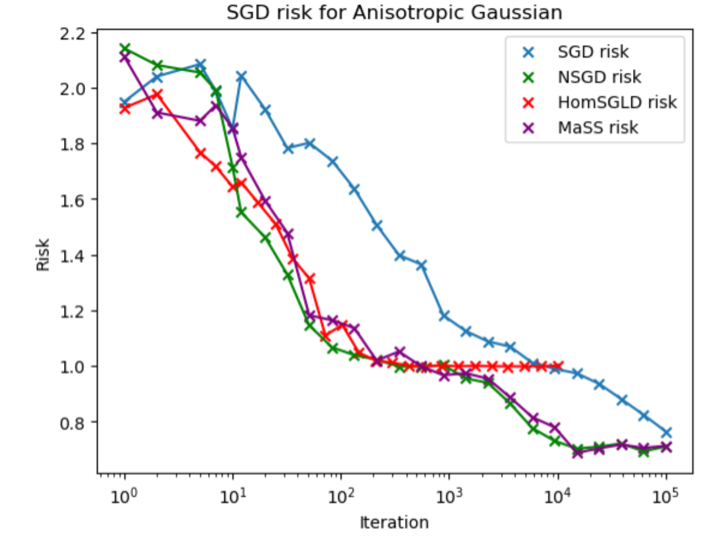
\includegraphics[width=.45\linewidth]{images/Nguyen2018-SGD-algos-risk-aniso-gauss.png}}\hfill
\subfloat[legend]{\label{b}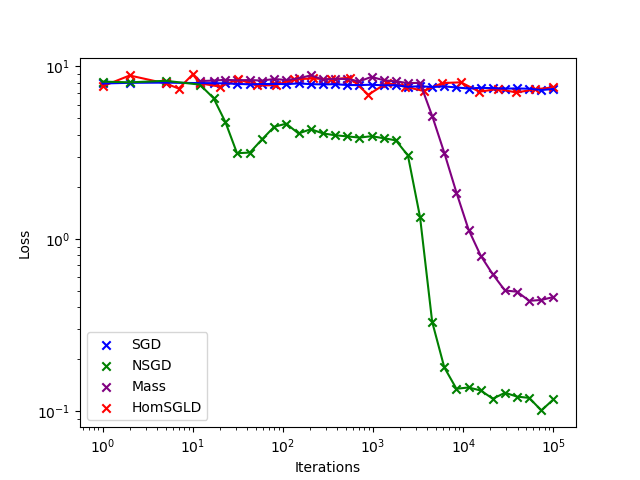
\includegraphics[width=.45\linewidth]{images/Nguyen2018-SGD-algos-risk-iso-gauss-non-mon.png}}\par 
\subfloat[legend]{\label{c}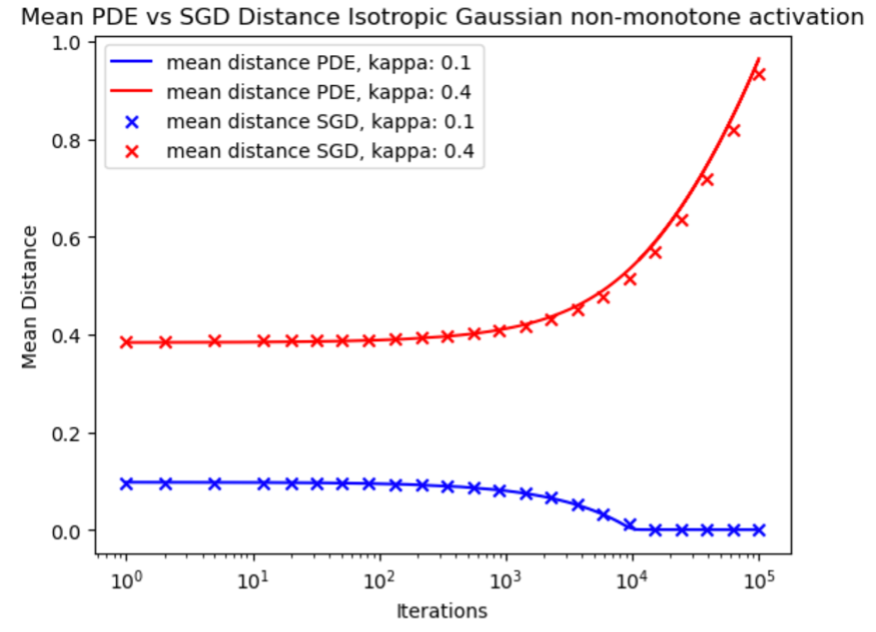
\includegraphics[width=.45\linewidth]{images/NGuyen2018-pde-sgd-iso-gauss-non-mon.png}}
\caption{my fig}
\label{fig}
\end{figure}


•	Isotropic Gaussian with non-monotone activation learning problem in the 2018 paper by Mei et al.
o	Here Nesterov accelerated and plain SGD were implemented
o	The non-monotone activation function in the neural network introduced some non-global minima where SGD seemed to get stuck, whereas Nesterov SGD seemed to avoid such ‘bad minima’ and attain monotonically decreasing losses characteristic of a global minimum. MF-HomSGLD seems to take longer to converge, maybe the hyper-parameters of the algorithm are not optimally tuned.
o	Here The MaSS algorithm seems to outperform the Nesterov accelerated sgd only in later iterations
 
 
•	3d-spin model considered in Vanden-Eijnden’s 2018 paper
o	In the deterministic gradient flow (with random initialization), the Nesterov accelerated loss (green) decreases  towards a minimum much faster than regular gradient descent (blue), as expected
 
o	In the stochastic gradient flow (with random initialization), the Nesterov accelerated loss (green) decreases  towards a minimum faster than regular gradient descent (blue), though the losses stay closer together
\begin{figure}[H]
  \centering
  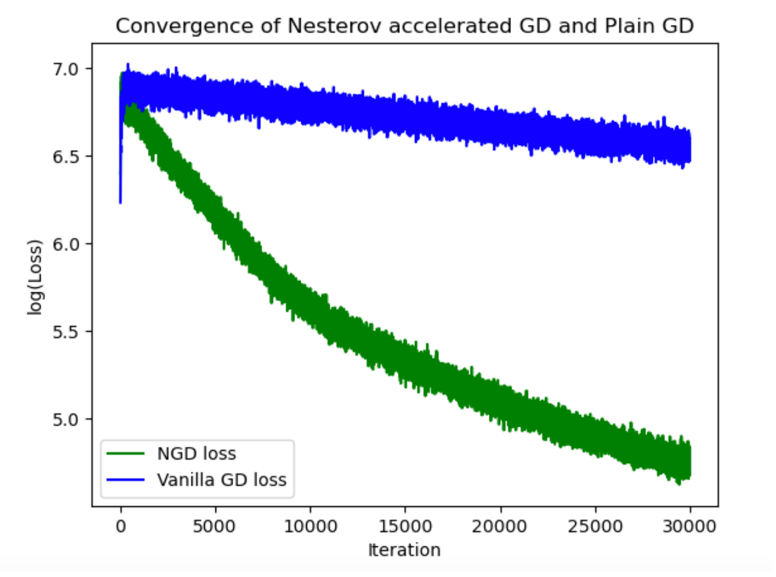
\includegraphics[width=0.8\textwidth]{images/Eijnden2018-SGD-algos-risk-3dspin.png}
  \caption{ caption}
  \label{fig: description}
\end{figure}%
 
•	Single-digit classification algorithm on the MNIST dataset
o	Nesterov acceleration beat plain SGD, but was beaten by MF-HomSGLD, which plateaued early but achieved a substantially smaller loss in the same amount of time
     \begin{figure}[H]
 \begin{subfigure}{0.5\textwidth}
   \centering
   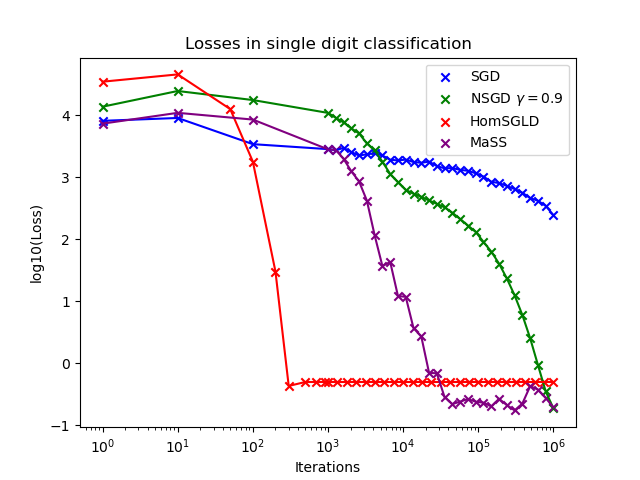
\includegraphics[width=0.8\linewidth]{images/Spiliopoulos2019-SGD-algos-single-digit classification.png}
   \caption{ caption}
   \label{fig: description}
 \end{subfigure}%
 \begin{subfigure}{0.5\textwidth}
   \centering
   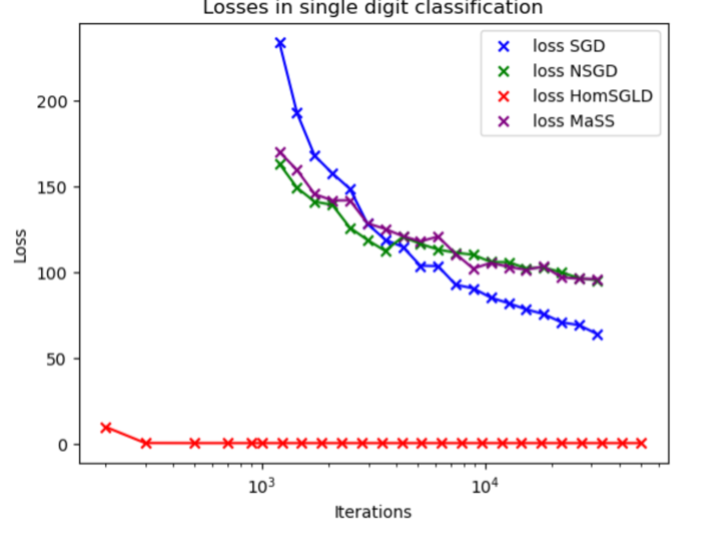
\includegraphics[width=0.8\linewidth]{images/Spiliopoulos2019-SGD-algos-single-digit-late-time.png}
   \caption{ caption}
   \label{fig:  description}
 \end{subfigure}
 \caption{ caption}
 \label{fig:  label}
 \end{figure} 
 
Some general observations: 
•	For Nesterov accelerated descent:
o	In the deterministic case, as showcased by the 3d-spin model, Nesterov clearly beats plain GD;  this is to be expected.
o	This acceleration is harder to see in the stochastic setting. Nesterov-accelerated SGD seems on all occasions to perform better than plain SGD, but in some cases marginally so.
o	The more noteworthy observation is that it gets ‘unstuck’ at the ‘bad’ minimum in the non-monotone activation case.
•	The MF-HomSGLD algorithm:
o	I chose to implement this algorithm because it corresponds to a discretisation of a gradient flow with respect to a regularized potential.
o	MF-HomSGLD matches the performance of plain SGD, but it seems to get stuck for larger iterations and plateaus. However in the MNIST one-digit classification, the algorithm attains a substantially smaller loss, about two orders of magnitude less than the other algorithms, but it suffers from plateauing early again.
•	The MaSS algorithm: 
o	In most cases, despite claims in the paper by Liu and Belkin of exponential convergence (assuming certain regularity restraints on the loss which may be optimistic in my case), the performance at least matches Nesterov SGD, since it is a perturbation thereof. However, in the non-monotone activation function case, it beats all algorithms in later iterations and descends the fastest in loss.

\newpage
\bibliographystyle{plain}
\bibliography{references}

\end{document}
